\chapter{Código}
\section{Funciones Auxiliares}
\subsection{void senal (int s)}
Función que se encarga de activar o desactivar las señales SIGINT y SIGQUIT, de tal modo que en caso de tratarse de un proceso en background o de la propia minishell, no respondan. Sin embargo no se activarán si es un proceso foreground.\\
Su funcionamiento es muy sencillo: usando la función \textit{signal} si se le pasa el parámetro 0 las desactiva, y si es un 1 las activa.
\subsection{void comandoCD(char* ruta)}
Mediante la función $chdir$ cambia el directorio de trabajo al especificado en "ruta". En caso de no especificar una ruta, accede a HOME. En caso de introducirse una ruta inexistente avisará del error.
\subsection{int** crearPipes (int n)}
Función que se encarga de crear las tuberías necesarias. Crea $n-1$ tuberías, puesto que para el último hijo no es necesario crear una tubería al ser éste el que ejecuta el último mandato.
\subsection{void cerrarPipes(int** pipes,int n)}
Método que cierra todas las tuberías usadas hasta ese momento.
\subsection{void liberarPipes(int** pipes,int n)}
Método que libera el espacio reservado de las tuberías usadas.
\subsection{int redirecEntrada (tline* linea)}
En caso de que se haya introducido un comando con el símbolo $<$ y se trate del primer mandato, se activará la redirección por entrada. Para ello abre el fichero con el nombre especificado por \textit{linea->redirect-input} con permisos de solo lectura, y si no hay error al leerlo copiará el contenido del fichero a la entrada estándar.
\subsection{int redirecSalida (tline* linea)}
En caso de que se haya introducido una orden con el símbolo $>$ y se trate del último comando, se activará la redirección por salida. Para ello se creará un fichero con el nombre especificado por \textit{linea->redirect-output} con permisos de lectura y escritura para todo el mundo, y si no hay error al crearlo copiará la salida estándar al fichero.
\subsection{int redirecError (tline* linea)}
Como en la función anterior, si en el último comando se introduce una orden con el símbolo $\&$ se activará la redirección por error. Para ello se creará un fichero con el nombre especificado por \textit{linea->redirect-error} con permisos de lectura y escritura para todo el mundo en el que guardará, en caso de error, la información sobre la misma.
\subsection{void falloEntrada (int descriptor,char* fichero)}
Función que comprueba si se ha cometido un fallo en la apertura de un fichero, y en tal caso, muestra el mensaje de error y finaliza el proceso hijo.
\subsection{void lectura (int* pipe)}
Este método recibe una tubería, y se encarga de cerrar el lado de escritura [1], duplicando el lado de lectura [0].
\subsection{void escritura (int* pipe)}
Este método recibe una tubería, y se encarga de cerrar el lado de lectura [], duplicando el lado de escritura [1].
\section{Main}
El método principal sigue un esquema similar al siguiente:
\begin{figure}[]
\begin{center}
 \centering
 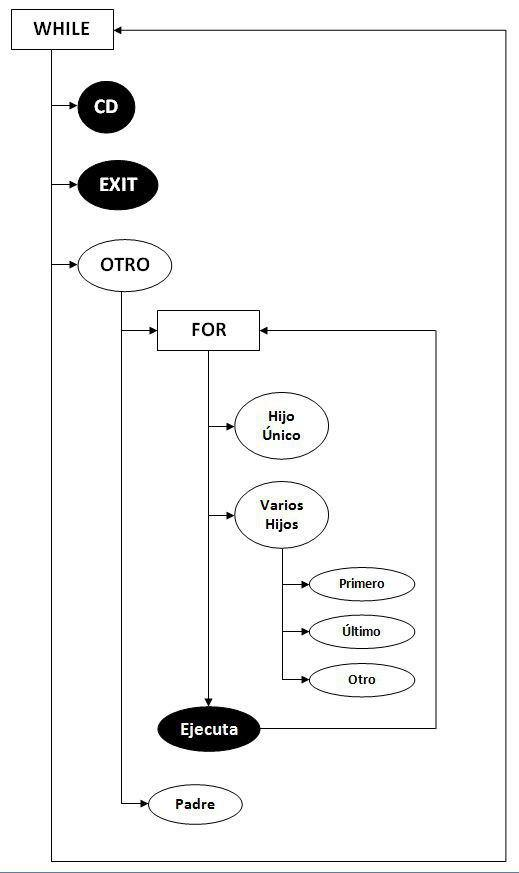
\includegraphics[width=0.8\textwidth]{./esquema}
 \caption{Esquema del main}
 \label{fig:Esquema del main}
\end{center}
\end{figure}
Explicamos muy brevemente su funcionamiento:
\newpage 
\begin{enumerate}
 \item WHILE: inicia un bucle infinito que lee por entrada estándar los comandos a ejecutar.
 \item CD: en el caso de que el primer comando introducido sea \textit{cd}, ejecutará el comando cd realizando una llamada al método auxiliar \textit{comandoCD}.
 \item EXIT: en el caso de que el primer comando introducido sea \textit{exit}, finalizará el programa.
 \item OTRO: en el caso de que el primer comando no sea ninguno de los dos anteriores, inicializará una lista de tuberías (con tantas tuberías como comandos-1 que posea la línea), e iniciar un bucle FOR con tantas iteraciones como comandos se hayan introducido, en la que en cada una se hace la llamada a \textit{fork()} bifurcando el proceso en proceso.
 \item HIJO ÚNICO: en el caso de que solo se haya introducido un solo comando, se redireccionará la entrada y salida (tanto normal como error), en caso de que venga indicado en el comando.
 \item VARIOS HIJOS: en el caso de que haya más de un comando, se procederá de la siguiente manera:
 \begin{itemize}
  \item PRIMERO: si el proceso bifurcado es el primero, se redireccionará la entrada, en caso de que venga indicado en el comando, y pondrá en modo escritura la primera tubería.
  \item ÚLTIMO: si el proceso bifurcado es el último, se redireccionará la salida (tanto la normal como error), en caso de que venga indicado en el comando, y se pondrá en modo lectura la última tubería.
  \item OTRO: si no es el primer o último comando, se pondrá la tubería anterior en modo lectura y la actual en modo escritura.
 \end{itemize}
 \item EJECUTA: sea cual sea el proceso bifurcado, se ejecutará el comando correspondiente, y en caso de que no se ejecute, se mostrará por pantalla el error de que el mandato no se ha encontrado, finalizando el proceso.
 \item PADRE: el proceso padre, en el caso de que el comando ejecutado se produzca en foreground, esperará a que terminen los comandos antes de proceder a mostrar el promp. En el caso de que el comando ejecutado se produzca en background, desactivará para este la señales SIGINT y SIGQUIT, mostrará el pid del proceso que se está ejecutando en background, y volverá a mostrar el prompt.
\end{enumerate}

\chapter{Comentarios personales}
\section{Problemas encontrados}
Al igual que la práctica anterior, hemos ido añadiendo funcionalidades de manera incremental. De esta manera, en un principio comprobamos el correcto funcionamiento al ejecutar un solo comando. A continuación probamos si es capaz de redireccionar la salida y la entrada correctamente, añadiendo posteriormente la funcionalidad para el comando "cd". Finalmente añadimos la comunicación entre procesos. Este último paso fue el que más problemas nos acarreó, ya que en un principio no poseíamos los conocimientos teóricos suficientemente claros y no sabíamos como debían crearse los procesos (si se crean hijos sucesivos, o se crean hijos hermanos). Además, nos dieron muchos problemas las tuberías, especialmente en el último proceso, ya que no se cerraba correctamente. Por ello tuvimos que añadir el método $cerrarPipes$ que cierra todas las tuberías anteriores, asegurándonos así que no nos cejábamos alguno abierto.\\
Además para ayudarnos a comprender el funcionamiento de nuestro código, creamos un archivo paralelo que realizaba las mismas funciones, pero mostrando por pantalla información útil para nosotros (pid en ejecución, estado de las pipes...) de los procesos actuales. Manejábamos dichos procesos mediante mandatos $sleep$, de forma que podíamos ver de forma tranquila y detallada el estado de nuestro programa.
\section{Posibles mejoras}
Debido a la falta de tiempo no hemos podido comprobar las fugas de memoria, así que no sabemos cual es la calidad de nuestro código en este aspecto. Por otra parte, se podrían continuar añadiendo funcionalidades a la shell hasta conseguir una similar a la original. Podríamos por tanto añadir antes del promp el usuario que ha ejecutado la terminal, o añadir la funcionalidad del autocompletado con la tecla tabulación, que facilita enormemente el uso de la terminal cuando hay que escribir rutas largas o tratar con nombres de archivos largos. Siguiendo con ampliaciones que mejoran el manejo de la shell, también ofrecer la posibilidad de usar las teclas de arriba y abajo para acceder al historial de comandos introducidos.\\
Por otro lado, la estructura de nuestro método $main$ no nos parece la más eficiente posible, ya que tiene un número muy alto de ramificaciones y, francamente, es complicado de entender hasta para nosotros. Por tanto nuestra primera prioridad si dispusiéramos de más tiempo sería cambiar la estructura del main, reduciendo todo lo posible las ramificaciones y añadiendo más métodos auxiliares que ayuden a la comprensión del código. 